%\documentclass[12pt,handout,xcolor=pdftex,dvipsnames,table]{beamer} %For handouts.
\documentclass[xcolor=pdftex,dvipsnames,table]{beamer}
% This is the file main.tex
\usepackage{pifont} %Symbols package
\usepackage{fixltx2e} % Superscript and subscript
\usepackage{hyperref} %\Url Links
\usepackage{cleveref}

\makeatletter
\newcommand\hyper@makecurrent[1]{}
\makeatother

\usepackage{caption} %caption for figures
%\usepackage[caption=false]{subfig}
\usepackage{subcaption} %subfigures
\usepackage{url}
\usepackage{multimedia}
\usepackage[final]{pdfpages}
\usepackage{textpos}
\usepackage{graphicx}
\usepackage[english]{babel}
\usepackage[utf8]{inputenc}
\usepackage[T1]{fontenc}
\usepackage{amsmath}
\usepackage{array} %\professional tables
\usepackage{lmodern}% http://ctan.org/pkg/lm (For special Fonts)

\mode<presentation>
\usetheme{Dresden} % so so
\setbeamertemplate{blocks}[rounded][shadow=true]
\setbeamertemplate{navigation symbols}{} %take out the navigation symbols
%\setbeamertemplate{caption}[numbered] %enumerate the caption and tables
\captionsetup{labelformat=simple}
%\numberwithin{figure}{section} %takes the figure number of the section e.g. Figure 3.1
\usefonttheme[stillsansseriflarge]{structureitalicserif}
\expandafter\def\expandafter\insertshorttitle\expandafter{%
  \insertshorttitle\hfill\insertframenumber\,/\,\inserttotalframenumber}%page numbering

%\makeatletter %reset the numbering on the subfigures (1)
%\@addtoreset{subfigure}{figure} %reset the numbering on the subfigures (2)
%\makeatother %reset the numbering on the subfigures (3)

%For Large figures
%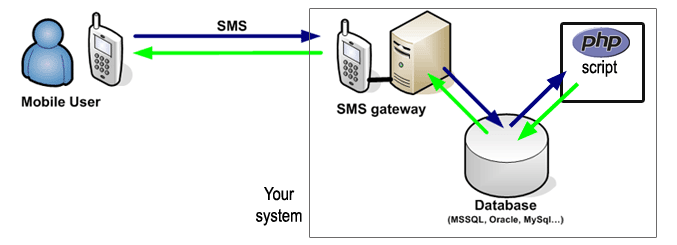
\includegraphics[width=\linewidth,height=\textheight,keepaspectratio]{SMS}

\title[Group 8] % (optional, only for long titles)
{QoEMoVi - QoE Based Cross-Layer Design of Mobile Video Systems}
\subtitle{ET2541 Advanced Topic in Telecommunication Systems}
\vspace*{-2.2em}
\author[Athanasios~Garyfalos, Eldin~Malko\v c]% (optional, for multiple authors)
{A.~Garyfalos \and E.~Malko\v c}
\institute[Blekinge Tekniska Högskola, Karlskrona. Sweden] % (optional)
{
\\
\medskip
{
\emph{A.atga12@student.bth.se}
\emph{B.elma09@student.bth.se}
}
}
\date[BTH 2013]{Presentation: 1, 2013}
\subject{Department of Computer Science}

\begin{document}

\begin{frame}[noframenumbering]
  \begin{center}
    % Upper part of the page
    % \vspace*{5.0em}
    
\includegraphics[width=.8\textwidth]{png/djangoRestLogo}\\ [0.3cm]    

    % \emph{Supervisor:} \\  
    % Prof.~Kulesza\\
    % \textsc{Wlodek} 
  \end{center}
  \titlepage
\end{frame}

\section*{Copyright Disclaimer}
  \begin{frame}
    \begin{justify}
      {\justifying Copyright \alert{Disclaimer}: This program is free software: you can redistribute it and/or modify it under the terms of the GNU General Public License as published by the Free Software Foundation, either version 3 of the License, or (at your option) any later version.
      \bigbreak
      This program is distributed in the hope that it will be useful, but WITHOUT ANY WARRANTY; without even the implied warranty of MERCHANTABILITY or FITNESS FOR A PARTICULAR PURPOSE.  See the GNU General Public License for more details.
      \bigbreak
      You should have received a copy of the GNU General Public License along with this program.  If not, see.~\cite{gnuLicences} }
    \end{justify}
\end{frame}

\section*{Contents}
\begin{frame}
\setbeamercovered{dynamic}%Makes the text appear before it presents nice!!!! 
\frametitle{Outline}
\tableofcontents[pausesections]
\end{frame}

\include{./technology_evolves/technology_evolves}
\include{./state_of_the_art/state_of_the_art}
\include{./currently_forefront/currently_forefront}
\section{Summary}
  \subsection{Key points repetition}

\begin{frame}
\setbeamercovered{dynamic}
  \begin{exampleblock}{Summary}
    \begin{itemize}[<+->]
      \item In section~``\nameref{sec:group}'' page ``\ref{sec:group}'' we mentioned member positions and responsibilities. 
      \item In section~``\nameref{sec:wireless}'' page ``\ref{sec:wireless}'' we mentioned hardware components and best/worst positions.
      \item In section~``\nameref{sec:implementation}'' page ``\ref{sec:implementation}'' we mentioned our approach and proposed solution to the problem \pause
    \end{itemize}
  \end{exampleblock}
  \begin{exampleblock}{Extra Notes}
    \begin{itemize}[<+->]
      \item Both the Conference paper and the Presentation where written in \alert{\LaTeX}
      \item Due to the quality of the output it exceeds our expectations!~\cite{research}
    \end{itemize}
  \end{exampleblock}
\end{frame}

\subsection*{Questions}
\begin{frame}
%\begin{overlayarea}{\textwidth}{3cm}
    %\only<1>{Some text for the first slide.\\Possibly several lines long.}
    %\only<2>{Replacement on the second slide.}
%\end{overlayarea}
  \begin{itemize}
     \Large
    \item \colorbox{yellow}{Thanks a lot – questions \& comments?}
  \end{itemize} 
\end{frame}

\section{Bibliography}
\subsection*{Web and Articles}

\begin{frame}[allowframebreaks]
  \frametitle<presentation>{References}
  \bibliographystyle{amsalpha}   
  \begin{thebibliography}{10}
    %\setbeamertemplate{bibliography item}[online]
    \setbeamertemplate{bibliography item}{
\includegraphics[width=1.5em]{./png/gnu}}
    \bibitem{gnuLicences}
      GNU LESSER GENERAL PUBLIC LICENSE
      \newblock {\emph{GNU Operating System}}
      \newblock available at \url{https://www.gnu.org/licenses/lgpl.html}.
    %\setbeamertemplate{bibliography item}[online]
    \setbeamertemplate{bibliography item}{
\includegraphics[width=1.5em]{./png/www}}
    \bibitem{djangoRestFramework}
      Author: T.~Christie
      \newblock {\emph{Django Rest Framework Project}}
      \newblock available at \url{http://www.django-rest-framework.org}.
    \setbeamertemplate{bibliography item}[article]
    \setbeamertemplate{bibliography item}{
\includegraphics[width=1.3em]{./png/heroku}}
    \bibitem{herokuApi}
      Author: A.~Garyfalos
      \newblock {\emph{thanos-test.herokuapp}}
      \newblock available at \url{https://thanos-test.herokuapp.com}.
  \end{thebibliography}
\end{frame}

\end{document}
